\documentclass{standalone}
\usepackage{graphicx}	
\usepackage{amssymb, amsmath}
\usepackage{color}

\usepackage{tikz}
\usetikzlibrary{intersections, backgrounds, math}
\usepackage{pgfmath}

\definecolor{light}{RGB}{220, 188, 188}
\definecolor{mid}{RGB}{185, 124, 124}
\definecolor{dark}{RGB}{143, 39, 39}
\definecolor{highlight}{RGB}{180, 31, 180}
\definecolor{gray10}{gray}{0.1}
\definecolor{gray20}{gray}{0.2}
\definecolor{gray30}{gray}{0.3}
\definecolor{gray40}{gray}{0.4}
\definecolor{gray60}{gray}{0.6}
\definecolor{gray70}{gray}{0.7}
\definecolor{gray80}{gray}{0.8}
\definecolor{gray90}{gray}{0.9}
\definecolor{gray95}{gray}{0.95}


\begin{document}

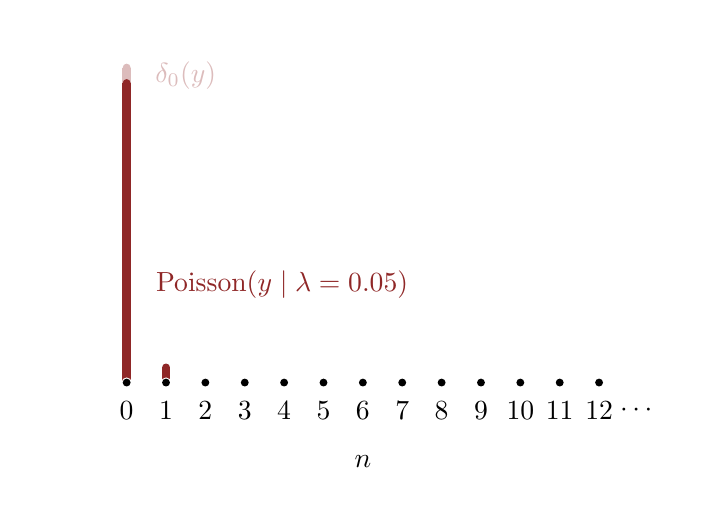
\begin{tikzpicture}[scale=1]
  \begin{scope}[shift={(0, 0)}]
    \draw[white] (-4.25, -3.5) rectangle (4, 2.5);
    
    \foreach [count=\n] \m in {1} {
      \pgfmathsetmacro{\x}{0.5 * ( (\n - 1) - 6)};
      \draw[light, line width=3] (\x, -2) -- (\x, {(4 * \m - 2)});
      \fill[light] (\x, {(4 * \m - 2)}) circle (0.05);
    }
    
    \node[light] at (-2.25, 1.9) { $\delta_{0}(y)$ };

    \foreach [count=\n] \m in {0.951, 0.048, 0.001, 0.000, 0.000, 0.000, 0.000, 0.000, 0.000, 0.000, 0.000, 0.000, 0.000} {
      \pgfmathsetmacro{\x}{0.5 * ( (\n - 1) - 6)};
      \draw[dark, line width=3] (\x, -2) -- (\x, {(4 * \m - 2)});
      \fill[dark] (\x, {(4 * \m - 2)}) circle (0.05);
      \fill[white] (\x, -2) circle (0.065);
      \fill[black] (\x, -2) circle (0.05);
      
      \pgfmathtruncatemacro{\nn}{\n - 1}
      \node at (\x, -2.35) { $\nn$ };
    }
    
    \node[dark, anchor=west] at (-2.75, -0.75) { $\mathrm{Poisson}(y \mid \lambda = 0.05)$ };
 
    %\fill[white] (3.5, -2) circle (0.06);
    %\fill[black] (3.5, -2) circle (0.05);
    \node at (3.5, -2.35) { $\cdots$ };
 
    \node at (0, -3) { $n$ };
  \end{scope}
  
\end{tikzpicture}

\end{document}  